
\title{PivotalR:\@ A Package for Machine Learning on Big Data}
\author{by Hai Qian}

\maketitle

% An abstract of less than 150 words
\abstract{ \pkg{PivotalR} is an R package that provides a front-end to
  PostgreSQL and all PostgreSQL-like databases such as Pivotal Inc.'s
  Greenplum Database (GPDB)~\citep{gpdb}, HAWQ~\citep{hawq}. When
  running on the products of Pivotal Inc., \pkg{PivotalR} utilizes the
  full power of parallel computation and distributive storage, and
  thus gives the normal R user access to big data. \pkg{PivotalR} also
  provides the R wrapper for MADlib. MADlib is an open-source library
  for scalable in-database analytics. It provides data-parallel
  implementations of mathematical, statistical and machine-learning
  algorithms for structured and unstructured data. Thus \pkg{PivotalR}
  also enables the user to apply machine learning algorithms onto big
  data.  }

\section{Introduction}

% Goals

% Similar products

% basic idea (SQL transfer)

% What it is: wrapper of database manipulation, wrapper of MADlib

In recent years, Big Data has become an important research topic and a
very realistic problem in industry. The amount of data that we need to
process is exploding, and the ability of analyzing big data has become
the key factor in competition. Big data sets do not fit into
computer's memory and it would be really slow if the big data sets
were processed sequentially. On the other hand, most contributed
packages of R are still strictly sequential, single machine, and they
are restricted to small data sets that can be loaded into memory. As
computing shifts irreversibly to parallel architectures and big data,
there is a risk for the R community to become irrelevant.

Some efforts have been invested into developing packages that give R
users and developers the access to some of the parallel distributive
platforms. Some examples include \pkg{dplyr}~\citep{dplyr},
\pkg{RHadoop}~\citep{RHadoop} (including \pkg{plyrmr}, \pkg{rmr},
\pkg{rhdfs}, \pkg{rhbase}), \pkg{RHIPE}~\citep{RHIPE},
\pkg{RHive}~\citep{RHive}, \pkg{teradataR}~\citep{teradatar} etc.

In this paper we introduce the package
\CRANpkg{PivotalR}~\citep{pivotalr}, which provides an R front-end
with data.frame oriented API for R users to access big data stored in
distributive databases or Hadoop distributive file system
(HDFS)~\citep{hdfs}. In this sense, \pkg{PivotalR} is close to the
still under development \pkg{dplyr} package, which has a data.frame
oriented API and multiple back-ends including several SQL database
systems.  \pkg{PivotalR} puts more emphasis on machine learning by
providing a wrapper for MADlib~\citep{madlib}, which is an open-source
library of scalable in-database machine learning algorithms. Actually
\pkg{PivotalR} offers more than what MADlib has. It adds
functionalities that do not exist in MADlib, for example, the support
for categorical variables. \pkg{PivotalR} makes it easier to work on
big data sets in databases.

This package is especially useful for users who are not familiar with
SQL language, because the functions and syntax for the manipulation of
tables are very similar to those for data.frame manipulation defined
natively in R. Thus the learning curve for the package is very smooth.
\pkg{PivotalR} is also very useful for users who are familiar with SQL
language, because it brings the graphical and analytical
functionalities of R to the processing of big data stored in
databases.

\pkg{PivotalR} is contributed to the open-source community by the
Predictive Analytics Team at Pivotal Inc\@. In order to gain the power
of distributive storage and parallel computation, the users need to
have a distributive database system installed, for example the
Greenplum Database or HAWQ\@. \pkg{PivotalR} also supports the
open-source database system PostgreSQL\@. Therefore \pkg{PivotalR}
benefits R users by providing an easy-to-access interface for
manipulating data tables stored in PostgreSQL database system and a
combination of the powers of R and MADlib, which lets the user
directly apply machine learning algorithms onto the big data stored in
databases.

It is worth mentioning that \pkg{PivotalR} provides the access to data
stored on HDFS by supporting HAWQ~\citep{hawq}, which is the SQL query
engine on HDFS created by Pivotal Inc.

The user does not need to worry about the restriction of memory size
even if the data size is very big, because \pkg{PivotalR} minimizes
the amount of data transferred between the database and R. The user
manipulates the data from R but the data itself stays in the database.

The work flow of using \pkg{PivotalR} is the following. First, the
user uses \code{"db.connect"} to connect to a database. Then,
\code{"db.data.frame"} can be used to create a wrapper for a data
table
in the database. Minimal information about the table is kept in the
wrapper, and no data is loaded into the memory. The user can easily
operate on the \code{"db.data.frame"} wrapper object and any operation
creates a
\code{"db.Rquery"} object, which is just a wrapper for a series of
operations and contains a SQL query string (see the section of
Manipulation of Data Tables in Database). During this data preparation
step, no data is loaded. In the next step, the user can either call
\code{"lookat"} function to view a sample of the operation result, or
call one of the MADlib wrapper functions to execute a machine learning
algorithm. Both choices initiates computation in the connected
database. Usually the computation result is small and can be loaded
into memory for further processing. In some cases, the result is also
big,
for example, the MADlib wrapper for ARIMA produces the residuals for
each row of the data. In such cases, a table is created in the
database to store the result and a wrapper is automatically created in
R, and the user can use the same work flow to analyze the result
table.

From the above work flow, one can see that all the actual computation
is done in the database. So the performance depends on the
database. For the Greenplum database or HAWQ, all computation is done
in a parallel and distributive way. Especially the MADlib machine
learning functions are all implemented to fully utilize the parallel
and distributive power of the databases. There are some operations
that cannot be done in a parallel way, for example the ordered
aggregate, but they have not been implemented in \pkg{PivotalR}
yet. For the Postgres database, even though the computation is not in
parallel, the user can still use PivotalR to easily access the data
stored in the database, which might be too big to load into
memory. Actually the performance on Postgres is not bad at all. In our
performance tests
in Postgres database, PivotalR's ARIMA wrapper function for MADlib is
faster than R's own \code{"arima"} function when applied onto large
data
sets.

It is worth mentioning that the Greenplum database (GPDB)~\citep{gpdb}
has a community edition, which is free (but not open-source) and has
all the functionalities except the technical support from Pivotal Inc.

At the time of writing, the version of \pkg{PivotalR} on CRAN is 0.1.8.

In this paper, we briefly introduce the usage of \pkg{PivotalR}. First
in the next section we explain the architecture of
\pkg{PivotalR}. Then we use various examples to illustrate the usage
and work flow of \pkg{PivotalR}.

\section{Architecture of \pkg{PivotalR}}

As is shown in Fig.~\ref{fig:structure}, \pkg{PivotalR} connects to
the database through the \CRANpkg{RPostgreSQL}~\citep{rpostgresql}
package. However, \pkg{PivotalR} does not directly call the functions
in RPostgreSQL. Instead we create an abstraction layer to wrap the
functions of RPostgreSQL, and the access to the database is done by
calling
the functions in the abstraction layer, which then call the functions
in RPostgreSQL. This design makes it easier to add supports for other
data storage platforms in the future. Right now, \pkg{PivotalR} only
supports the connection to PostgreSQL, GPDB (Greenplum Database) and
HAWQ. Through HAWQ, \pkg{PivotalR} can access the big data stored on
HDFS.

In the future, \pkg{PivotalR} will add supports to other DBMS, Pivotal
HD (Hadoop created by Pivotal Inc.)  and Hadoop (MapReduce), but we
have not decided about how to do that. This is why there are question
markers in Fig.~\ref{fig:structure}.

The table operation functions are built upon the abstraction layer for
accessing data. The syntax of these functions is the same as R's
\code{"data.frame"} operation functions, such as \code{[, [<-, \$,
  \$<-}, \code{merge}, \code{"by"} etc. Arithmetic methods such as
\code{+, -, *, /}, logical functions such as \code{>, <, ==, !=, <=,
  >=, !, |, \&}, math functions such as \code{log, exp, factorial}
etc. are all implemented.

The layers that are built upon the table operations are the MADlib
function wrappers and
other functions, which will be covered in the subsequent sections.

A graphical user interface using the \CRANpkg{shiny}~\citep{shiny}
package is also implemented. Right now it only provides the graphical
interface to the MADlib wrapper functions, but we have the plan to
provide the
graphical access to all functionalities of \pkg{PivotalR} in the
future.

\begin{figure}[htb]
  \centering
  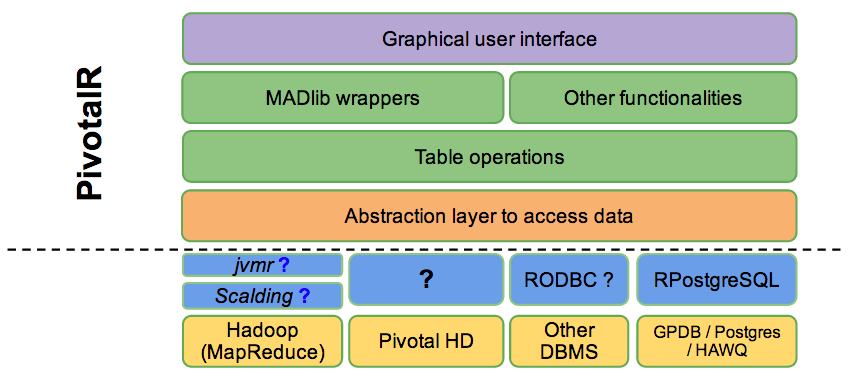
\includegraphics[width=0.85\textwidth]{PivotalR_structure.png}
  \caption{The structure of \pkg{PivotalR}. \pkg{PivotalR} accesses
    the data storage through an abstraction layer which wraps the
    functions that can directly access the database. Other types of
    data storages will be supported in the future. Right now it only
    supports connections to PostgreSQL, GPDB and HAWQ. Table
    operations functions are built upon the data accessing layer. They
    have the exact same interface as R's \code{"data.frame"} operation
    functions. MADlib function wrappers and other functions are built
    upon the table operations. The graphical user interface makes the
    package easier to use.}
\label{fig:structure}
\end{figure}

It is worth explaining more about how \pkg{PivotalR} operates on the
tables. Before everything, the user needs to create a
\code{"db.data.frame"} object, which is just a wrapper of the
table. Any operation on this object is translated into an SQL query
string. However, the SQL query is not executed at this point, and is
instead stored in an object of class \code{"db.Rquery"} in R. When the
user wants to execute the operation, he can call the function
\code{"preview"} or \code{"lookat"} (or a shorthand \code{"lk"}) to
execute
the operation and load part
or all of the results into memory to view. The user can also choose to
use \code{"as.db.data.frame"} to execute the SQL query and save the
result into a new table. This design gives the user the freedom to
choose when to load data into memory or create tables to store
intermediate data in the process of a calculation. It also avoids the
risk of accidentally loading big data into memory.

In order to realize the above design, we use a class hierarchy shown
in Fig.~\ref{fig:hierarchy}. \pkg{PivotalR} uses S4 object-oriented
programming extensively. All objects that are related to the data in
the database belong to subclasses of an abstract class named
\code{"db.object"}.

\begin{figure}[htb]
  \centering
  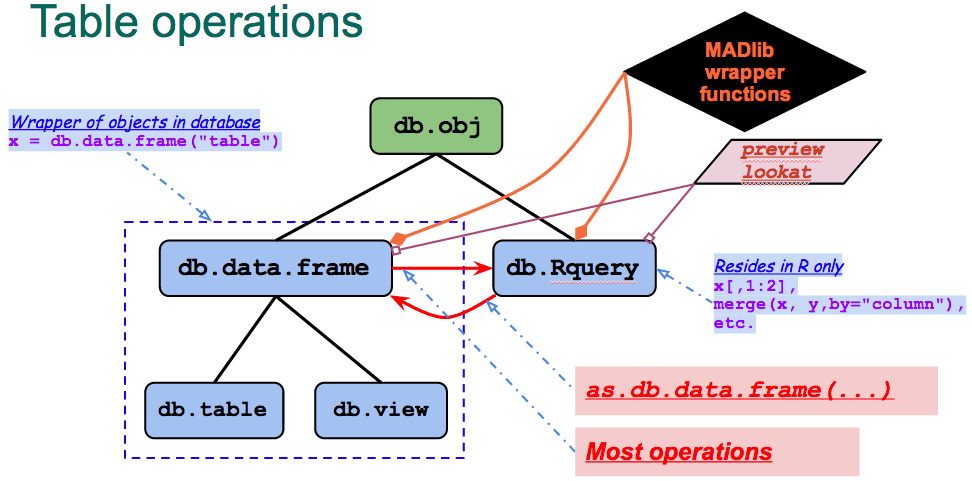
\includegraphics[width=0.9\textwidth]{class-hierarchy.png}
  \caption{The class hierarchy of \pkg{PivotalR}. This is not a UML
    figure. The square blocks represent the S4 classes. The arrows
    represent the conversion between the classes. The dashed arrows
    represent the various operations that convert the classes. The
    MADlib wrapper functions and preview/lookat function operate on
    both db.data.frame class and db.Rquery class.}
\label{fig:hierarchy}
\end{figure}

As has been mentioned, the class \code{"db.data.frame"} is a wrapper
of data objects stored in the connected database. When it is created
by the command \code{"db.data.frame"}, no actual data stored in the
data table in the database is transferred from the database to R. This
object just contains some basic information about the data object in
the database, such as dimensions and column
names. \code{"db.data.frame"} has two sub-classes, \code{"db.table"}
and \code{"db.view"}, which are wrappers for tables and views
respectively.

\begin{example}
> library(PivotalR)
> conn.id <- db.connect(port = 14526, dbname = "madlib", host =
+                       "localhost")
Created a connection to database with ID 1
> x <- db.data.frame("abalone")
\end{example}

The command \code{"db.connect"} in the abstraction layer is used to
connect to one or multiple databases. It has an optional parameter
that lets the user select which package he wants to use to connect to
the databases, although only \pkg{RPostgreSQL} is supported right
now. The returned value of \code{"db.connect"} is an integer which
represents the database connection.  \pkg{PivotalR} can connect to
multiple databases at the same time. Thus it is possible to train a
machine learning model using the data from database 1 and then make
predictions using the data from database 2. One can use
\code{"db.disconnect"} to disconnect a connection and \code{"db.list"}
to list all active connections.

Any operation on an object of the class \code{"db.data.frame"}
produces an object of the class \code{"db.Rquery"}. An object of the
class \code{"db.Rquery"} resides entirely on the R side, and is a
wrapper of operations on a \code{"db.data.frame"} object. Most
operations on a \code{"db.Rquery"} object produces another
\code{"db.Rquery"} object. Essentially, a \code{"db.Rquery"} object is
just a container of a string of SQL query, which can be viewed using
the command
\code{"content"}.  The command \code{"as.db.data.frame"} creates a
table
in the database using the results of the SQL query contained in a
\code{"db.Rquery"} object and then creates a \code{"db.data.frame"}
wrapper that points to this table.

\code{"preview"} (or its alias \code{"lookat"} and \code{"lk"})
transfers the data
from
the database into R's memory. By default it fetches $100$ rows of data
from the table in the database and convert the data into
\code{"data.frame"} in R.

\begin{example}
> lookat (x, 10)
   id sex length diameter height  whole shucked viscera shell rings
1   4   M  0.440    0.365  0.125 0.5160  0.2155  0.1140 0.155    10
2   8   F  0.545    0.425  0.125 0.7680  0.2940  0.1495 0.260    16
3  12   M  0.430    0.350  0.110 0.4060  0.1675  0.0810 0.135    10
4  16   M  0.500    0.400  0.130 0.6645  0.2580  0.1330 0.240    12
5  20   M  0.450    0.320  0.100 0.3810  0.1705  0.0750 0.115     9
6  24   F  0.550    0.415  0.135 0.7635  0.3180  0.2100 0.200     9
7  28   M  0.590    0.445  0.140 0.9310  0.3560  0.2340 0.280    12
8  32   F  0.680    0.560  0.165 1.6390  0.6055  0.2805 0.460    15
9  36   M  0.465    0.355  0.105 0.4795  0.2270  0.1240 0.125     8
10 40   M  0.355    0.290  0.090 0.3275  0.1340  0.0860 0.090     9
\end{example}

The MADlib wrappers can be applied onto both \code{"db.data.frame"}
and \code{"db.Rquery"} objects. When a MADlib wrapper function is
applied onto a \code{"db.Rquery"} object, a temporary table is created
using \code{as.db.data.frame}. MADlib is an in-database
library and we have to convert \code{"db.Rquery"} into an object
inside the database so that we could apply MADlib functions onto
it. This temporary table is dropped after the computation is done.

The design of \pkg{PivotalR} minimizes the amount of data that needs
to be transferred between the database and R. The only function that
transfers data from the database is \code{"preview}.

\section{Manipulation of Data Tables in Database}

As has been mentioned, \pkg{PivotalR} overloads many methods that
operate on \code{"data.frame"}, and thus lets the operations on the
\code{"db.obj"} objects mimic those on \code{"data.frame"} as much as
possible.

\begin{example}
> x <- db.data.frame ("abalone")
> dim (x)
[1] 4177   10
> names (x)
 [1] "id"       "sex"      "length"   "diameter" "height"   "whole"
 [7] "shucked"  "viscera"  "shell"    "rings"
> x$rings <- x$rings + 2 / 3
> x$newCol <- (x$rings + x[['length']]) < 10
> content(x)
[1] "select \"id\" as \"id\", \"sex\" as \"sex\", \"length\" as \"length\",
\"diameter\" as \"diameter\", \"height\" as \"height\", \"whole\" as \"whole\",
\"shucked\" as \"shucked\", \"viscera\" as \"viscera\", \"shell\" as \"shell\",
(\"rings\")::double precision + 0.666666666666667 as \"rings\",
(((\"rings\")::double precision + 0.666666666666667)::double precision
+ (\"length\"))::double precision < 10 as \"newCol\" from \"abalone\""
\end{example}
Here \code{"content"} displays the SQL query stored in the
\code{"db.Rquery"}. The quotes inside the SQL query is used to deal
with column or table names with special characters. \code{x} was
originally a \code{"db.data.frame"} object, but was converted to a
\code{"db.Rquery"} object by the operation \code{x\$rings <- x\$rings
  +
  2 / 3}.

As long as a \code{"key"} is specified when the user calls
\code{"db.data.frame"} function, the syntax \code{A[3,4]} can be used.
Here the first number \code{"3"} means that the key column has the
value of \code{3}. Therefore, \code{lk(A[3,4],-1)} may return multiple
values. This is different from the behavior of \code{"data.frame"},
where \code{A[3,4]} returns the element on 3-rd row and 4-th column.
This difference is related to the lack of intrinsic order in the
database tables, which will be discussed in the following.

The operations on \code{"db.obj"} objects mimic those on
\code{"data.frame"}. However, there is important difference between
\code{"db.obj"} and \code{"data.frame"}.

The rows of a \code{"data.frame"} object have an intrinsic order,
which makes the operations that involve two \code{"data.frame"}
objects easier to define. For example, it is straightforward to define
the subtraction of two columns of two different \code{"data.frame"}
objects by matching the order of the rows as long as they have the
same number of rows.

On the other hand, the tables in the database do not have an intrinsic
order for the rows. Thus, most operations like subtraction, addition
etc.\ can only be defined for columns belonging to the same
table. However, this is usually not a problem. Whenever the user wants
to do an operation that involves two tables, he/she should first
call the function \code{"merge"} to create a new table (actually a
\code{"db.Rquery"} object) from the two
tables and at the same time explicitly specify how to match the rows
of the two different tables. Then, the user can easily do operations
on the new table. While R's \code{"data.frame"} implicitly uses the
intrinsic order of the rows to match the rows from two different
data.frames, this needs to be explicitly done for
\code{"db.data.frame"}
objects. For example,
\begin{example}
> x <- db.data.frame("abalone")
> y <- db.data.frame("abalone")
> z <- merge(x, y, by = NULL) # cross join two tables
> names(z)
 [1] "id_x"       "sex_x"      "length_x"   "diameter_x" "height_x"
 [6] "whole_x"    "shucked_x"  "viscera_x"  "shell_x"    "rings_x"
[11] "id_y"       "sex_y"      "length_y"   "diameter_y" "height_y"
[16] "whole_y"    "shucked_y"  "viscera_y"  "shell_y"    "rings_y"
> z$sex_x == z$sex_y # This is a db.Rquery object
\end{example}

The data frame \file{abalone} is lazy-loaded in \pkg{PivotalR}. It is
used as an example data here. One can use \code{as.db.data.frame} to
transfer this data set into a table in the database and at the same
time create a wrapper for the table

\begin{example}
> x <- as.db.data.frame(abalone, conn.id=1)
The data in the data.frame abalone is stored into the table in database madlib on localhost !
\end{example}

All the subsequent operations will be applied onto the table wrapper
\code{x}. A sample of the data is shown in the following, where
\code{sort} is used to create a sorting operation on the original
table.
\begin{example}
> lookat(sort(x, FALSE, x$id), 10) # load 10 rows of the sorted data
   id sex length diameter height  whole shucked viscera shell rings
1   1   M  0.455    0.365  0.095 0.5140  0.2245  0.1010 0.150    15
2   2   M  0.350    0.265  0.090 0.2255  0.0995  0.0485 0.070     7
3   3   F  0.530    0.420  0.135 0.6770  0.2565  0.1415 0.210     9
4   4   M  0.440    0.365  0.125 0.5160  0.2155  0.1140 0.155    10
5   5   I  0.330    0.255  0.080 0.2050  0.0895  0.0395 0.055     7
6   6   I  0.425    0.300  0.095 0.3515  0.1410  0.0775 0.120     8
7   7   F  0.530    0.415  0.150 0.7775  0.2370  0.1415 0.330    20
8   8   F  0.545    0.425  0.125 0.7680  0.2940  0.1495 0.260    16
9   9   M  0.475    0.370  0.125 0.5095  0.2165  0.1125 0.165     9
10 10   F  0.550    0.440  0.150 0.8945  0.3145  0.1510 0.320    19
\end{example}

At last, I want to reiterate that all these operations done on
\code{"db.data.frame"} are not executed immediately. Instead a
\code{"db.Rquery"} object is produced. The user can
convert it into a real table using \code{as.db.data.frame}.

\section{MADlib Wrapper Functions}

In the next, we show some examples of MADlib wrapper functions. As is
shown in Fig.~\ref{fig:hierarchy}, all MADlib wrapper functions can be
applied onto \code{"db.obj"} objects. Because the connection
information is already contained in \code{"db.obj"} objects, we do not
need to specify \code{"conn.id"} in the MADlib wrapper functions.

First, we show several examples of linear regression. Basically,
\pkg{PivotalR}'s \code{"madlib.lm"} uses the same formula syntax as
\code{"lm"}. Because MADlib's linear regression supports fitting
separate linear regression models on sub-groups of the data, which are
grouped by one or multiple columns, \code{"madlib.lm"} allows
\code{"|"}
in the formula, which means that the model is fit on a subset of the
data conditioned on the value of the variables after \code{"|"}.

\begin{example}
> ## fit one different model to each group of data with the same sex
> fit <- madlib.lm(rings ~ . - id | sex, data = x)
\end{example}

\code{sex} has $3$ distinct values, and thus \code{fit} is a list of 3
elements. Each element is the linear regression model for a subset of
the data. The mean square error can be easily computed

\begin{example}
> ## apply the model onto data in another database
> lookat(mean((x$rings - predict(fit, x))^2)) # mean square error
  rings_madlib_predict_opr_opr_avg
1                         4.647291
\end{example}

We can plot a random sample of the fitting values together with the
real values, as is shown in Fig.~\ref{fig:sample}. We can also select
one model from the fitting result to plot, as is shown in the comments
of the following snippets.

\begin{example}
> ## plot the result
> ap <- cbind(x$rings, predict(fit, x)) # combine two columns
> plot(lookat(sort(ap, FALSE, NULL), 100)) # plot a random sample
> ## ap <- cbind(x$rings[x$sex == "I"], predict(fit[[1]], x[x$sex == "I",]))
> ## plot(lookat(sort(ap, FALSE, NULL), 100)) # plot a random sample
\end{example}

\begin{figure}[htb]
  \centering
  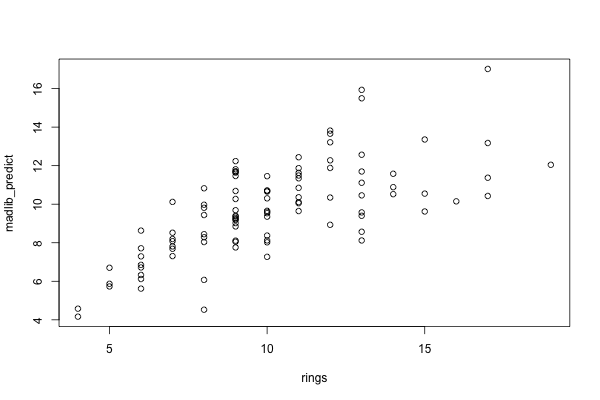
\includegraphics[width=0.85\textwidth]{sample_plot.png}
  \caption{The sample plot}
  \label{fig:sample}
\end{figure}

The support to categorical variables is done through
\code{"as.factor"}, as is shown in the next example.

\begin{example}
> v <- x
> v$sex <- as.factor(v$sex) # specify which column to pivot
> f <- madlib.lm(rings ~ . - id, data = v)
> f
MADlib Linear Regression Result

Call:
madlib.lm(formula = rings ~ . - id, data = v)

---------------------------------------

Coefficients:
             Estimate Std. Error  t value       Pr(>|t|)
(Intercept)   3.89464    0.29157  13.3576  6.992e-40 ***
sex:M         0.05772    0.08335   0.6925  4.887e-01
sex:I        -0.82488    0.10240  -8.0558  1.022e-15 ***
length       -0.45834    1.80912  -0.2533  8.000e-01
diameter     11.07510    2.22728   4.9725  6.876e-07 ***
height       10.76154    1.53620   7.0053  2.861e-12 ***
whole         8.97544    0.72540  12.3730  1.469e-34 ***
shucked     -19.78687    0.81735 -24.2086 2.988e-121 ***
viscera     -10.58183    1.29375  -8.1792  3.757e-16 ***
shell         8.74181    1.12473   7.7723  9.639e-15 ***
---
Signif. codes:  0 '***' 0.001 '**' 0.01 '*' 0.05 '.' 0.1 ' ' 1

R-squared: 0.5378844
Condition Number: 137.2694
\end{example}

Because \code{extractAIC} method is implemented for the result of
\code{madlib.lm} and \code{madlib.glm}, one can use R's \code{step}
function for feature selection.
\begin{example}
  fit <- madlib.glm(rings<10 ~ ., data = x, family = "binomial")
  step(fit)
\end{example}
This is a good example of how R's analytical functionalities can be
combined with MADlib.

In the next example, we use the bootstrap aggregate method to fit a
linear model to the data.

\begin{example}
  ## generic bagging
  fit <- generic.bagging(function(data) {
                            madlib.lm(rings ~ . - id - sex, data = data)
                         },
                         data = x, nbags = 10, fraction = 0.85)

  pred <- predict(fit, newdata = x) # make prediction

  lookat(mean((x$rings - pred)^2))
\end{example}

Just like \code{"glm"} in \CRANpkg{stats}~\citep{stats} package,
\pkg{PivotalR} provides \code{"madlib.glm"}, which can do both linear
and logistic regressions. The usage is similar to \code{glm}. Please
refer to \pkg{PivotalR} manual \citep{pivotalr} for details.

\section{Support for Array Columns}

Both Greenplum database and Postgres database have an upper limit for
the number of columns in a data table. The upper limit depends on the
column data types, but is usually around 1600. If the big data set has
more features, the only workaround is to use an array column to
encapsulate all the features, because there is no limit for how many
elements an array can contain.

\pkg{PivotalR} has the full support for such array columns, as is
shown in the next example.

\begin{example}
> z <- db.data.frame("madlibtestdata.lin_auto_mpg_oi")
> lookat(z, 10)
   x.1 x.2 x.3 x.4 x.5 x.6 x.7  y
1     8  383  170 3563 10.0   70    1 15
2     8  340  160 3609  8.0   70    1 14
3     8  400  150 3761  9.5   70    1 15
4     4  121  113 2234 12.5   70    2 26
5     8  360  215 4615 14.0   70    1 10
6     8  304  193 4732 18.5   70    1  9
7     4  113   95 2228 14.0   71    3 25
8     6  250   88 3302 15.5   71    1 19
9     8  351  153 4154 13.5   71    1 14
10    8  318  150 4096 13.0   71    1 14
> madlib.lm(y ~ x, data = z)
MADlib Linear Regression Result

Call:
madlib.lm(formula = y ~ x, data = z)

---------------------------------------

Coefficients:
              Estimate Std. Error t value      Pr(>|t|)
(Intercept) -17.218435   4.644294 -3.7074 2.402e-04 ***
x[1]         -0.493376   0.323282 -1.5261 1.278e-01
x[2]          0.019896   0.007515  2.6474 8.445e-03 **
x[3]         -0.016951   0.013787 -1.2295 2.196e-01
x[4]         -0.006474   0.000652 -9.9288 7.883e-21 ***
x[5]          0.080576   0.098845  0.8152 4.155e-01
x[6]          0.750773   0.050973 14.7288 3.069e-39 ***
x[7]          1.426140   0.278136  5.1275 4.666e-07 ***
---
Signif. codes:  0 '***' 0.001 '**' 0.01 '*' 0.05 '.' 0.1 ' ' 1

R-squared: 0.8214781
Condition Number: 85850.33
\end{example}

\section{Handling of NULL Values}

\pkg{PivotalR} makes it very easy to filter \code{NULL} values from a
table. Here we show an example using the data \code{"null.data"} comes
with \pkg{PivotalR}. \file{null.data} has lots of \code{NULL} value.
However, we can easily
filter out all the \code{NULL} values.

% deal with NULL values
\begin{example}
> delete("null_data", conn.id = 2)
[1] TRUE
> w <- as.db.data.frame(null.data, "null_data", conn.id = 2)
The data in the data.frame null.data is stored into the table null_data in database madlib on localhost !
> dim(w)
[1] 67126    10
> lookat(w, 10)
   sf_mrtg_pct_assets ris_asset lncrcd lnauto lnconoth lnconrp intmsrfv
1               31.62    208596      0     NA    18260      44        0
2               20.66     34647      0     NA     2997       0        0
3               14.95    160175      0     NA    15164       0        0
4               17.49    117398      0     NA    12365       0        0
5               35.59    233592      0     NA     6261     151        0
6               11.57    166387      0     NA    36356       0        0
7               10.56    102891      0     NA     6311       0        0
8                6.05     30138      0     NA     2664       0        0
9               14.53   1615727      0     NA    80829    1106      105
10              12.88     83090      0     NA    11815       0        0
   lnrenr1a lnrenr2a lnrenr3a
1        NA       NA       NA
2        NA       NA       NA
3        NA       NA       NA
4        NA       NA       NA
5        NA       NA       NA
6        NA       NA       NA
7        NA       NA       NA
8        NA       NA       NA
9        NA       NA       NA
10       NA       NA       NA
> db.objects("null", conn.id = 2)
[1] "madlibtestdata.credit_nulls"         "madlibtestdata.rf_golf_nullclass"
[3] "madlibtestdata.rf_nursery_nullclass" "madlibtestdata.table_has_null"
[5] "public.null_data"
> for (i in 1:10) w <- w[!is.na(w[i]),] # filter NULL values
> dim(w)
[1] 6789   10
> madlib.lm(sf_mrtg_pct_assets ~ ., data = w)
MADlib Linear Regression Result

Call:
madlib.lm(formula = sf_mrtg_pct_assets ~ ., data = w)

---------------------------------------

Coefficients:
              Estimate Std. Error   t value      Pr(>|t|)
(Intercept)  1.528e+01  1.471e-01 103.90694 0.000e+00 ***
ris_asset    1.602e-08  1.141e-08   1.40440 1.602e-01
lncrcd      -1.608e-07  7.725e-08  -2.08170 3.741e-02 *
lnauto      -3.871e-07  3.447e-07  -1.12301 2.615e-01
lnconoth    -7.498e-07  4.370e-07  -1.71559 8.628e-02 .
lnconrp      7.575e-08  1.229e-06   0.06165 9.508e-01
intmsrfv     8.609e-06  1.790e-06   4.81005 1.542e-06 ***
lnrenr1a    -4.827e-06  3.837e-05  -0.12580 8.999e-01
lnrenr2a     1.358e-04  2.359e-05   5.75605 8.986e-09 ***
lnrenr3a    -3.133e-05  4.273e-06  -7.33355 2.502e-13 ***
---
Signif. codes:  0 '***' 0.001 '**' 0.01 '*' 0.05 '.' 0.1 ' ' 1

R-squared: 0.01083685
Condition Number: 37854014
\end{example}

\code{na.action} is supported by \code{madlib.lm}, \code{madlib.glm}
and \code{madlib.elnet}. The user can define his own
\code{"na.action"} function. \code{"na.omit"} method is also
implemented.

\section{Quickly Creating Prototypes of Machine Learning Algorithms}

One of the goals of \pkg{PivotalR} is to help data scientists quickly
create prototypes for parallel machine learning algorithms that can
run in distributive databases. Although \pkg{PivotalR} is still at an
early stage of development, we already invest some effort into this.
The idea is to
implement some basic operations that forms the build blocks for most
machine learning algorithms.

For example, we implemented the function \code{crossprod}, which
computes the operation $X^{T}Y$. $X$ and $Y$ are wrappers created by
\code{"db.data.frame"} for tables that represent matrices. $X$ has $m$
rows (observations) and $n$ columns (features). The assumption here is
that $m$ can be very large but the number of features $n$ is
small. Thus results of $X^TX$ and $X^TY$ are both small and can be
loaded into memory for further calculations. The big data computation
only involves the computations of $X^TX$ and $X^TY$ in the database.

\begin{example}
  ## linear regression
  linregr <- function (x, y)
  {
    a <- crossprod (x)
    b <- crossprod (x, y)
    solve (lookat (a)) %*% lookat(b)
  }

  linregr (db.array(1, x[,-c (1,2,10)]), x[["rings"]])
\end{example}

Another example is the implementation of PCA for a matrix $Z$. Again
we assume that the number of columns $n$ is not large and the product
$Z^TZ$ is small enough to be loaded into memory. \pkg{PivotalR}
implements \code{"scale"}, which is used together with
\code{crossprod}
in this example.

\begin{example}
  ## PCA
  ## compute all eigenvectors in parallel
  ## can be used for tables with features < 1000

  pca <- function (x, center = TRUE, scale = FALSE)
  {
    y <- scale(x, center = center, scale = scale) # centering and scaling
    z <- as.db.data.frame(y, verbose = FALSE) # create an intermediate
    # table to speed up computation
    m <- lookat(crossprod(z)) # one scan of the table to compute Z^T * Z
    d <- delete(z) # delete the intermediate table
    res <- eigen(m) # only this computation is in R
    n <- attr(y, "row.number") # save the computation to count rows

    ## return the result
    list(val = sqrt(res$values/(n-1)), # eigenvalues
    vec = res$vectors, # columns of this matrix are eigenvectors
    center = attr(y, "scaled:center"),
    scale = attr(y, "scaled:scale"))
  }

  dat <- db.data.frame("madlibtestdata.pca_mat_600_100", conn.id = 2)

  q <- pca(dat[,-1])

\end{example}

\section{GUI of \pkg{PivotalR}}

As a front-end to both the database and MADlib, \pkg{PivotalR} also
provides a graphical user interface (GUI) to let users that are not
familiar with data science have an easy access to  the
functionalities. The GUI is written using the package \pkg{shiny},
which provides a very nice web application framework to create
graphical user interface.

The GUI is launched by the command \code{pivotalr} after the
connection to the databases have been created.
Fig.~\ref{fig:gui_table} and Fig.~\ref{fig:gui_linregr} show the
graphical user interface. Fig.~\ref{fig:gui_table} shows the screen
shot for the summary of various properties for all columns of a
table. The actual computation is done through MADlib's
\code{"summary"} function, which has a wrapper function
\code{"madlib.summary"} in \pkg{PivotalR}. Fig.~\ref{fig:gui_linregr}
shows the computation result of linear regression. The actual
computation is done through MADlib's \code{linregr\_train} function,
which has a wrapper function \code{"madlib.lm"}.

\begin{figure}
 \centering
  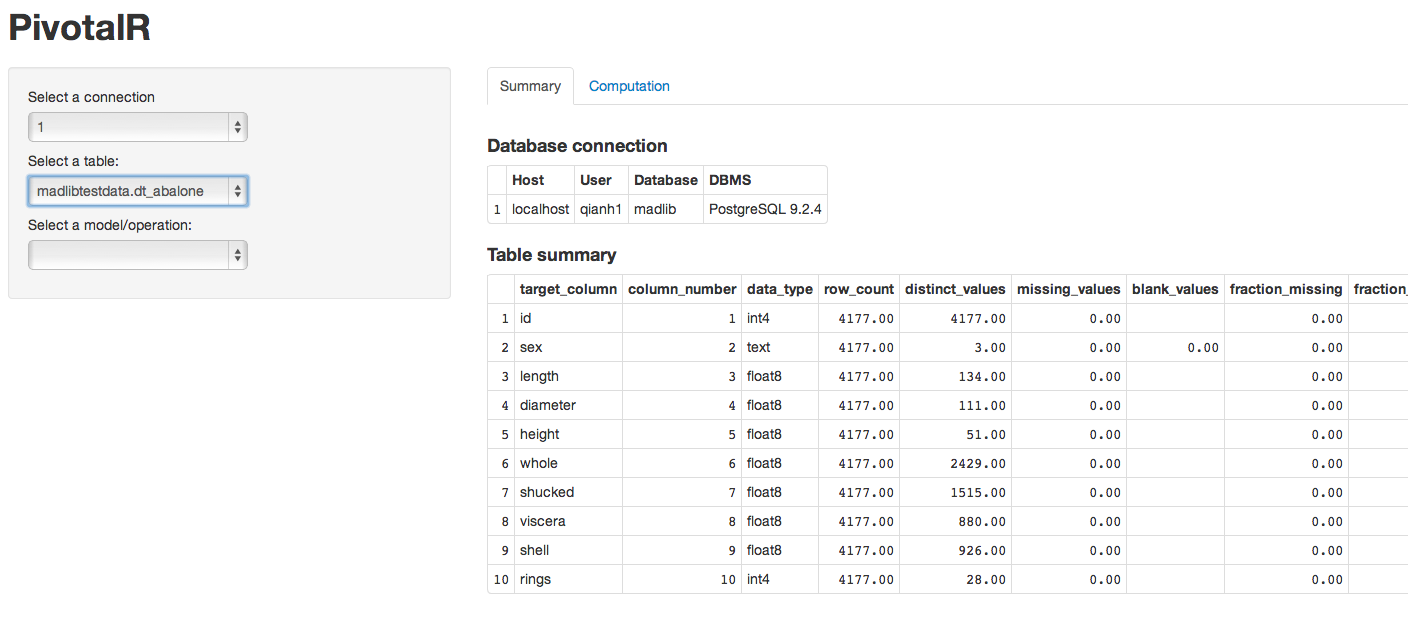
\includegraphics[width=0.85\textwidth]{gui_table.png}
  \caption{Display the summary of a table in the graphical interface.}
\label{fig:gui_table}
\end{figure}

\begin{figure}
 \centering
  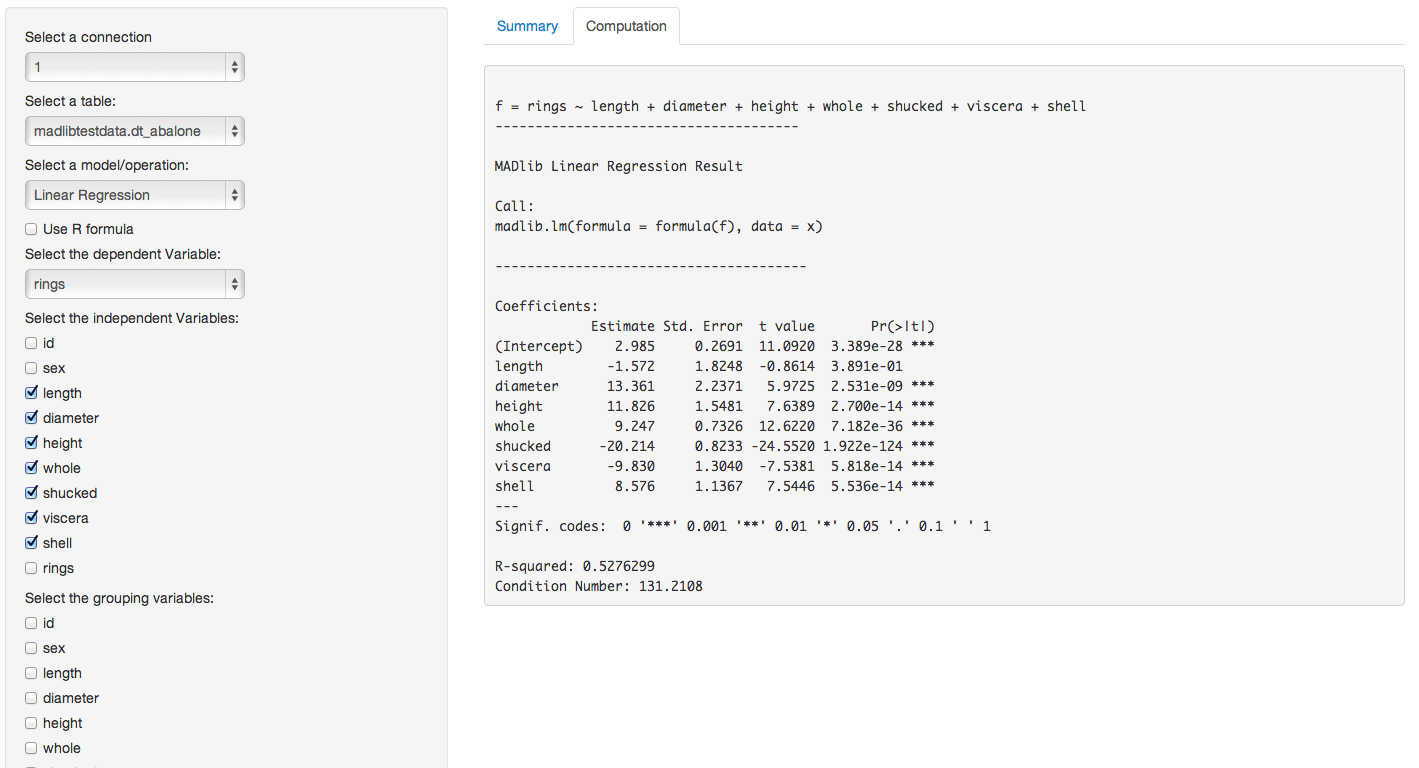
\includegraphics[width=0.85\textwidth]{gui_linregr.png}
  \caption{Display the result of linear regression in the graphical interface.}
\label{fig:gui_linregr}
\end{figure}

The GUI of \pkg{PivotalR} is based upon the package \pkg{shiny}, which
is a web application framework. Therefore the command \code{pivotalr}
launches a web application. One can run the GUI on the server and
connect to it using his web browser.

The GUI of \pkg{PivotalR} is still at its early development
stage. Many functionalities, especially the various operations on data
tables, cannot be done through GUI.\@ However, we expect to improve
the GUI gradually in the future releases.

\section{Future Work}
MADlib has a wide variety of machine learning functions.  At the time
of writing, the version of \pkg{PivotalR} on CRAN is 0.1.8, and it
implements 5 wrapper functions: linear regression, logistic
regression, ARIMA, elastic net regularization, and the data table
summary function. In the future, all MADlib functions will have their
wrappers in \pkg{PivotalR}. This is our highest priority right now.

As to the shiny interface of \pkg{PivotalR}, we are still exploring
the possibilities of streamlining the machine learning work flow and
making it compatible with a graphical interface. This by itself is a
big project, but it has a lower priority in our road-map.

The support for other platforms, like Hadoop or other database systems, is
also on our road-map, but has a relatively low priority too.

\section{Summary}

Here we introduced \pkg{PivotalR}, a package created by Pivotal
Inc. This package provides an R front-end to PostgreSQL and all
PostgreSQL-like databases like Pivotal Inc.'s Greenplum Database
(GPDB), HAWQ. \pkg{PivotalR} allows the user to manipulate tables in
database from within R. It also provides the wrapper functions for
MADlib,
which is an in-database machine learning library. \pkg{PivotalR}
implements the support for array columns and \code{NULL} handling. It
also helps the user quickly create prototypes of machine learning
algorithms. A graphical user interface based on shiny is also
implemented. In general, \pkg{PivotalR} gives the user the access to
big data stored in databases and an easy-to-use machine learning
toolkit.

\bibliography{qian}

\address{Hai Qian\\
  Pivotal Inc.\\
  3495 Deer Creek Rd., Palo Alto, CA 94304\\
  USA}
\email{hqian@pivotal.io}

